%% SYMBOLS AND ABBREVIATIONS
\section{Preliminaries}


\subsection{Big O notation}

 The Big O is a notation describing the execution time of an algorithm, either through memory or time usage. It is the asymptotic upper bound of a function that describes the algorithm. In computer science the Big O notation is used to analyze the time and space complexity of algorithms. and The Big O notation is a function of \inlineMath{n}, where \inlineMath{n} is the number of items handled in the algorithm. Described informally using the equation \inlineMath{f(n) = O(g(n))}, \inlineMath{f(n)} is smaller than some constant multiplied with \inlineMath{g(n)}.

 \begin{definition}
 We write \inlineMath{f(n) = O(g(n))}, if there exists a constant
 \inlineMath{c > 0} and \inlineMath{k > 0}, such that \inlineMath{0 \leq f(n) \leq cg(n) \: \forall \: n \geq k}
 \end{definition}
\subsection{Distributed system}

A distributed system is a set of networked computers, which coordinate their actions through communicating by messages. A distributed system can be modelled as a single coherent system. We can define this system as a set of nodes, connected in a network, that collectively coordinate and execute tasks.

Let the communication network of the distributed system be a graph \inlineMath{G = (V, E)}, where \inlineMath{V} is the set of vertices (or nodes), meaning the computing entities, or processes, of the system and \inlineMath{E} is the set of edges in the system that make up the communication links between the edges.

Each individual node, or process, in the set of nodes \inlineMath{V} has an internal state \inlineMath{S_p = (x_p, y_p)}, where \inlineMath{x_p} is a one-bit \emph{input register} and \inlineMath{y_p} a one-bit \emph{output register} with values in \inlineMath{\{b, 0, 1\}}. Let the state of the system be  \inlineMath{S = (S_1, S_2, ...., S_N)}. The behaviour of the system can be a set of rule of how the nodes interact with each other, altering the individual internal states of nodes and edges. These rules can be formalized as a set of functions \inlineMath{F}, that map the current state of the system \inlineMath{S} to a new state \inlineMath{S'}.

Define a distributed system as a tuple \inlineMath{(V, E, S, F)}, where \inlineMath{V} is the set of vertices (or nodes), \inlineMath{E} is the set of communication links between nodes, \inlineMath{S} is the current state of the system and \inlineMath{F} is the set of functions that define the behaviour of the system.

\subsection{Consensus problem}

The consensus problem asks to design a protocol that requires all computing entities, called agents, in a system, to agree on a binary value. This system of agent may include faulty agents, that may fail or produce faulty messages. The challenge is to make all non-faulty agents to have a shared understanding of the binary value in question, even with the presence of faulty agents. 

In order to reach consensus, each node in the set \inlineMath{V}, which is the set of nodes in the system, begins by \emph{proposing} the value in it's \emph{input register} \inlineMath{x_p}. Let the value proposed be \inlineMath{v_i}. The nodes then communicate and share their initial proposals. The nodes then decide on a decision value \inlineMath{d_i} and sets it in their respective \emph{output registers} \inlineMath{y_p}. The nodes are now in the \emph{decided state}, from which they can no longer return nor change the value of \inlineMath{y_p}. The requirements of a consensus algorithm are that, for each execution of it, these conditions should hold:

\begin{itemize}[label={}]
  \item \emph{Termination:} All correct nodes eventually sets the value of their output register and reach a decided state.
  \item \emph{Agreement:} All correct nodes share the same value in their output registers: if \inlineMath{V_i} and \inlineMath{V_j} are correct nodes and are in the \emph{decided state}, their corresponding states \inlineMath{S_i} and \inlineMath{S_j} share the same \emph{output register} values \inlineMath{y_i = y_j}.
  \item \emph{Integrity:} If all correct nodes proposed the same value, then any correct node that is in the \emph{decided state} has chosen that value.
\end{itemize}


%% Insert explanation on the graph below
In Figure \ref{fig:ConsensusProblem} we can see an example of the explanation above. Two nodes propose \emph{proceed} and the third node proposes \emph{abort}, but crashes thereafter. The two correct nodes that remain decide on \emph{proceed}.
\begin{figure}[H]
    \centering
    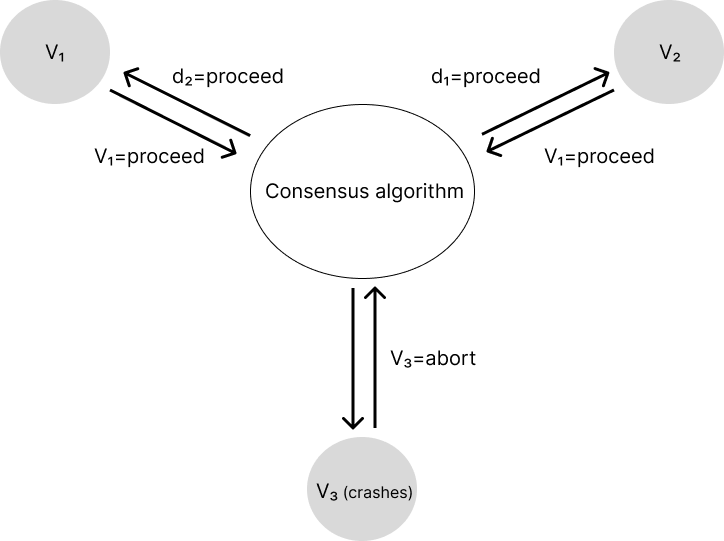
\includegraphics[width = 0.7\textwidth]{figures/consensus_problem.png}
    \caption{TODO caption}
    \label{fig:ConsensusProblem}
\end{figure}


Fault tolerance

\subsection{Asynchronous and synchronous systems}

Explain async and sync envs. Impossibility result in both envs

\subsection{Population protocols}



\subsection{Opinion dynamics}


% \linus{formal definitions of key concepts and notations. e.g. DS, DC problem, population protocols. Check Lynch survey}